% UV Builder logo -- hard-hat variant.
% A builder's hard hat shines a purple (UV) light on a Feynman diagram, inside a
% circle that opens for the hat at the top and for the name at the bottom.
% Compile with: pdflatex UVBuilderHatLogo.tex
\documentclass[tikz,border=6pt]{standalone}
\usepackage[T1]{fontenc}
\usepackage{tgpagella} % Palatino (TeX Gyre Pagella)
\usetikzlibrary{arrows.meta,fadings,decorations.pathmorphing,decorations.markings}

\definecolor{uvpurple}{RGB}{118,40,200}
\definecolor{uvindigo}{RGB}{42,14,88}

% ---------------------------------------------------------------------------
% Parameters (lengths in cm; the circle is centred on the origin)
% ---------------------------------------------------------------------------
\def\inkColor{uvindigo}      % hat, circle, diagram lines, "Builder"
\def\accentColor{uvpurple}   % light, photon, "UV", bottom wiggle
% --- circle ---------------------------------------------------------------------
\def\circleR{5}
\def\circleWidth{4pt}
\def\circleTop{138}          % the side arcs run from this angle (top) ...
\def\circleSide{211}         % ... down to this one (just above the text); mirrored on the right
\def\circleBottom{238}       % bottom arcs: from this angle ...
\def\circleWiggle{259}       % ... to this one, where the wiggle takes over; mirrored
% --- hat ------------------------------------------------------------------------
\def\hatY{3.75}              % height of the base of the dome
\def\domeW{2.2}              % half-width of the dome
\def\domeH{2.4}              % height of the dome
\def\hatStroke{7pt}
\def\brimW{3.1}              % half-width of the brim
\def\brimY{3.1}              % height of the brim tips
% --- light ----------------------------------------------------------------------
\def\lightTop{0.75}          % half-width of the light under the brim
\def\lightBottom{3.4}        % half-width at the bottom
\def\lightEnd{-2.7}          % where the light has faded out
\def\lightOpacity{0.8}
% --- diagram --------------------------------------------------------------------
\def\diagramWidth{5.4}
\def\diagramY{-0.6}          % height of the photon line
\def\diagramLineWidth{3pt}
% --- text -----------------------------------------------------------------------
\def\textY{-3.9}             % baseline
\def\textSize{1.7}           % font size, in cm

% ---------------------------------------------------------------------------
% Feynman diagram (same as in UVBuilderLogo.tex): s-channel e+ e- -> gamma -> e+ e-,
% total width `diagram width`, photon in `photon color`; centred on the pic origin
% ---------------------------------------------------------------------------
\tikzset{
  diagram width/.store in=\uvbDiagramWidth, diagram width=4cm,
  photon color/.store in=\uvbPhotonColor,   photon color=uvpurple,
  fermion/.style={postaction={decorate},
    decoration={markings, mark=at position 0.55 with {\arrow{Stealth[scale=1.4]}}}},
  antifermion/.style={postaction={decorate},
    decoration={markings, mark=at position 0.55 with {\arrowreversed{Stealth[scale=1.4]}}}},
  pics/diagram/.style={code={
    \coordinate (-in-e)  at (-0.5*\uvbDiagramWidth,-0.3*\uvbDiagramWidth);
    \coordinate (-in-p)  at (-0.5*\uvbDiagramWidth, 0.3*\uvbDiagramWidth);
    \coordinate (-out-e) at ( 0.5*\uvbDiagramWidth, 0.3*\uvbDiagramWidth);
    \coordinate (-out-p) at ( 0.5*\uvbDiagramWidth,-0.3*\uvbDiagramWidth);
    \coordinate (-v1)    at (-\uvbDiagramWidth/6,0);
    \coordinate (-v2)    at ( \uvbDiagramWidth/6,0);
    \draw[fermion]     (-in-e) -- (-v1);
    \draw[antifermion] (-in-p) -- (-v1);
    \draw[fermion]     (-v2) -- (-out-e);
    \draw[antifermion] (-v2) -- (-out-p);
    \draw[color=\uvbPhotonColor, decorate,
          decoration={snake, amplitude=0.025*\uvbDiagramWidth,
                      segment length=\uvbDiagramWidth/18}]
      (-v1) -- (-v2);
  }},
}

\begin{document}
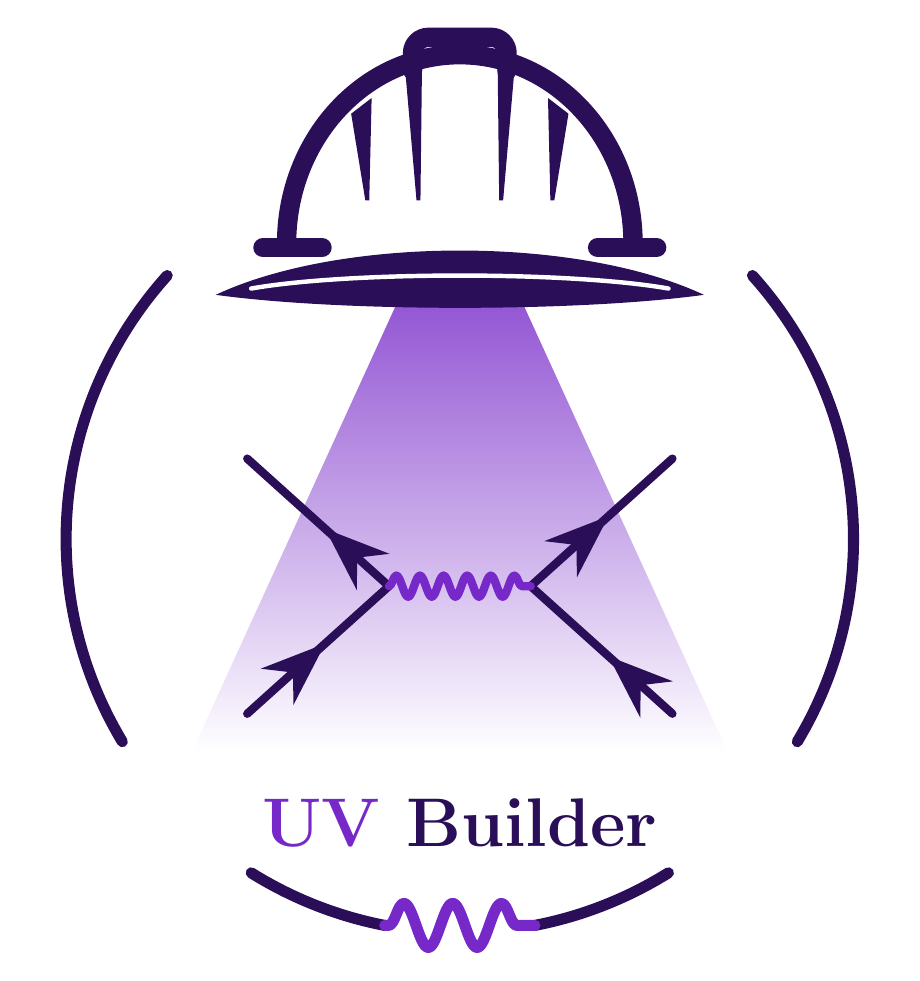
\begin{tikzpicture}[line cap=round, line join=round]

  % ---- light from under the brim (behind everything else) -------------------------
  \begin{scope}
    \clip (0,0) circle[radius=\circleR];
    \fill[\accentColor, fill opacity=\lightOpacity, path fading=south]
      (-\lightTop,\brimY) -- (\lightTop,\brimY)
      -- (\lightBottom,\lightEnd) -- (-\lightBottom,\lightEnd) -- cycle;
  \end{scope}

  % ---- circle: two side arcs, two bottom arcs, and a wiggle in the middle ------------
  \begin{scope}[draw=\inkColor, line width=\circleWidth]
    \draw (\circleTop:\circleR) arc[start angle=\circleTop, end angle=\circleSide, radius=\circleR];
    \draw ({180-\circleTop}:\circleR)
      arc[start angle={180-\circleTop}, end angle={180-\circleSide}, radius=\circleR];
    \draw (\circleBottom:\circleR)
      arc[start angle=\circleBottom, end angle=\circleWiggle, radius=\circleR];
    \draw ({540-\circleBottom}:\circleR)
      arc[start angle={540-\circleBottom}, end angle={540-\circleWiggle}, radius=\circleR];
  \end{scope}
  \draw[\accentColor, line width=\circleWidth, decorate,
        decoration={snake, amplitude=0.28cm, segment length=0.62cm,
                    pre length=0.05cm, post length=0.05cm}]
    (\circleWiggle:\circleR) -- ({540-\circleWiggle}:\circleR);

  % ---- hard hat ---------------------------------------------------------------------
  \begin{scope}[\inkColor]
    % dome, with a small foot on each side
    \draw[line width=\hatStroke]
      ({-\domeW},\hatY) arc[start angle=180, end angle=0, x radius=\domeW, y radius=\domeH];
    \draw[line width=\hatStroke]
      ({-\domeW-0.3},{\hatY-0.05}) -- ({-\domeW+0.45},{\hatY-0.05})
      ({\domeW+0.3},{\hatY-0.05}) -- ({\domeW-0.45},{\hatY-0.05});
    % raised ridge on top
    \draw[line width=\hatStroke, rounded corners=0.2cm]
      (-0.6,{\hatY+\domeH-0.2}) -- (-0.6,{\hatY+\domeH+0.22})
      -- (0.6,{\hatY+\domeH+0.22}) -- (0.6,{\hatY+\domeH-0.2});
    % tapering ribs: two along the ridge, one on each side
    \foreach \sx in {-1,1} {
      \fill ({\sx*0.48},{\hatY+\domeH-0.1}) -- ({\sx*0.7},{\hatY+\domeH-0.12})
            -- ({\sx*0.55},{\hatY+0.55}) -- ({\sx*0.5},{\hatY+0.55}) -- cycle;
      \fill ({\sx*1.12},{\hatY+\domeH-0.55}) -- ({\sx*1.38},{\hatY+\domeH-0.75})
            -- ({\sx*1.2},{\hatY+0.55}) -- ({\sx*1.15},{\hatY+0.55}) -- cycle;
    }
    % brim: a flat lens, with a thin highlight so it reads as a rim
    \fill (-\brimW,\brimY)
      .. controls (-1.5,{\brimY+0.75}) and (1.5,{\brimY+0.75}) .. (\brimW,\brimY)
      .. controls (1.5,{\brimY-0.22}) and (-1.5,{\brimY-0.22}) .. cycle;
    \draw[white, line width=1.6pt]
      ({-\brimW+0.45},{\brimY+0.08})
      .. controls (-1.4,{\brimY+0.3}) and (1.4,{\brimY+0.3}) .. ({\brimW-0.45},{\brimY+0.08});
  \end{scope}

  % ---- Feynman diagram ----------------------------------------------------------------
  \pic[\inkColor, line width=\diagramLineWidth, diagram width=\diagramWidth cm,
       photon color=\accentColor] at (0,\diagramY) {diagram};

  % ---- name ---------------------------------------------------------------------------
  \node[anchor=base, inner sep=0pt,
        font=\rmfamily\bfseries\fontsize{\textSize cm}{\textSize cm}\selectfont]
    at (0,\textY) {\textcolor{\accentColor}{UV} \textcolor{\inkColor}{Builder}};
\end{tikzpicture}
\end{document}
